\chapter{Diversidad de rango}
\label{cap.diversidad}

Los resultados del capitulo anterior, fueron complementados tras mencionar a los préstamos acumulados de un mismo campo semántico, cuyo rango descendió en un periodo de tiempo. Sin embargo, estas palabras no conforman todo el corpus de los préstamos acumulados; no se sabe lo que ocurre con el rango de los demás préstamos, al transcurrir el tiempo. 

Ya que los préstamos acumulados están organizados por año, y a la vez en cada año se ordenan las palabras de forma ascendente en rango, entonces a lo largo del tiempo, un mismo rango puede ser ocupado por diferentes palabras. 

La \textbf{diversidad de rango}, es un método para cuantificar la cantidad de elementos diferentes, que tienen un mismo rango dentro de un mismo corpus. El algoritmo para llegar a la diversidad, se describe en \cite{tesis.sergio} de la siguiente manera.


\begin{enumerate}
		
	\item Se fija el año inicial y el número de años $\Delta t$, a evaluar.
	
	\item Se toma el primer rango de todos los años a evaluar, y se cuenta el número de palabras distintas que aparecen en ese rango.  
	
	\item Se sigue con el segundo rango, y se vuelven a contar cuantas palabras distintas aparecen en él durante el periodo de tiempo. 
	
	\item El procedimiento anterior se repite para el número de rangos $k$ que se deseen o los que permita la base de datos. 
	
	\item Se normalizan los valores al dividir cada resultado entre $\Delta t$, obteniendo así la diversidad de rango $d(k)$.
	
\end{enumerate}

La diversidad de rango, ha sido empleada en bases de datos de las palabras más usadas por distintos idiomas \cite{iplosone}, y en diferentes clasificaciones de deportes y juegos \cite{epj}. Aunque se tratan de diferentes bases de datos, en ambos casos hay un resultado común: los rango más bajos son ocupados por una menor cantidad de palabras, y conforme aumenta el rango, también lo hace la cantidad de palabras que lo ocupan.

Se esperan obtener resultados similares en los préstamos acumulados, ya que estos son un subconjunto de las palabras más usadas por los idiomas. 

\section{Diversidad de rango de los préstamos acumulados}

Tras aplicar el algoritmo de la diversidad en cada pareja de idioma origen e idioma receptor, los valores se asemejan a una curva logarítmica.  A partir de esta distinción, se propone que la curva que mejor ajusta a la diversidad de rango $d(k)$, es de la forma:
\begin{equation}
\label{ec.ajuste} 
d(k) =  \alpha \ln(k) + \beta. 
\end{equation}
Donde los parámetros $\alpha$ y $\beta$  se  obtienen a través de una regresión lineal, entre los puntos obtenidos y la ecuación propuesta. 

Una vez calculados los parámetros $\alpha$ y $\beta$ de cada pareja de idiomas, se comprobó la fiabilidad del ajuste a partir del coeficiente de determinación $R^{2}$. Si $a_{k}$  representa el valor de la ecuación de ajuste al evaluarla en el rango $k$,  $d_{k}$ es la diversidad obtenida para el mismo rango y $\bar{d}$ es el promedio de todos los valores de la diversidad, entonces $R^{2}$ queda expresado como:
\begin{equation}
R^{2} = 1 - \sum_{k = 1} \frac{ \left( \,d_{k} - a_{k} \,\right)^{2}  }{ \left( \, d_{k} - \bar{d} \,\right)^{2} }.	
\label{ec.r2_diversidad}
\end{equation}
La tabla~\ref{tab.diversidad_ajuste} muestra el valor de $R^{2}$ de cada pareja de idiomas. 

  

\begin{table}[t]
	\centering
	\begin{tabular}{lcccccc}
		\multicolumn{7}{c}{R E C E P T O R}                                                                                                                                             \\
		\multirow{6}{*}{\begin{tabular}[c]{@{}l@{}}O\\ R\\ \,I\\ G\\ E\\ N\end{tabular}} &             & \textbf{inglés} & \textbf{francés} & \textbf{alemán} & \textbf{italiano} & \textbf{español}    \\
		& \textbf{inglés}   & -     & 0.94  & 0.92  & 0.92  & 0.89  \\
		& \textbf{francés}  & 0.93  & -     & 0.87  & 0.83  & 0.86  \\
		& \textbf{alemán}   & 0.85  & 0.90  & -     & 0.92  & 0.95  \\
		& \textbf{italiano} & 0.86  & 0.84  & 0.91  & -     & 0.91  \\
		& \textbf{español}  & 0.88  & 0.79  & 0.80  & 0.95  & -          
	\end{tabular}
	\caption{Fiabilidad del ajuste de la diversidad de rango, a partir del coeficiente de determinación $R^{2}$.}
	\label{tab.diversidad_ajuste}
\end{table}


\begin{figure}[h!]
	\centering
	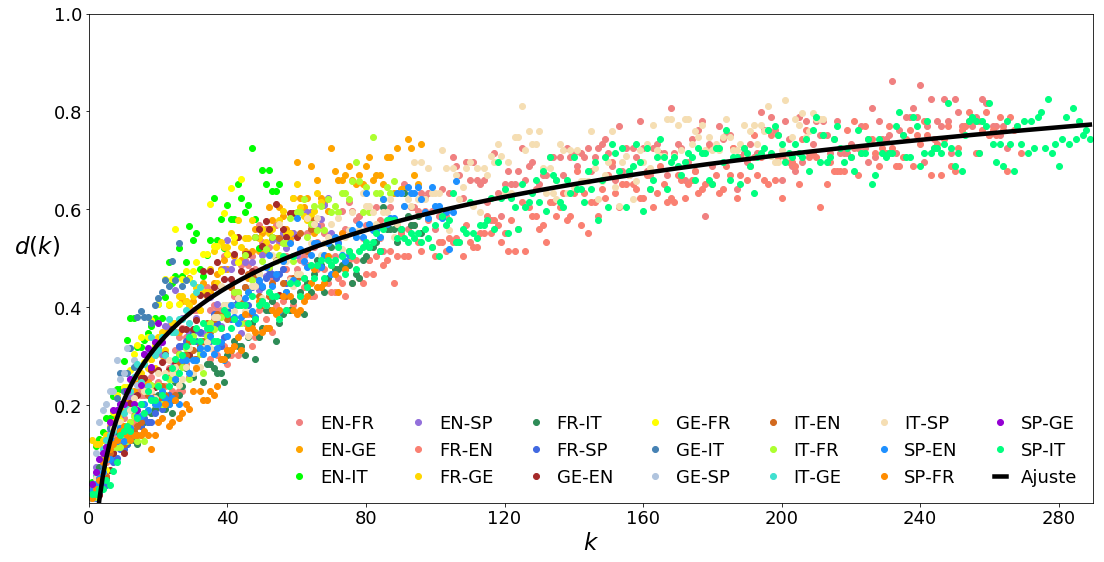
\includegraphics[scale=.38]{DR_gen.png}
	\caption{Diversidad de rango de los préstamos acumulados entre idiomas. Todas las parejas de idiomas muestran un comportamiento logarítmico, sin importar la cantidad de rangos donde se buscó la diversidad. En promedio, la fiabilidad  del ajuste de las 20 combinaciones a una ecuación logarítmica es de $R^{2}= 0.88 \pm 0.04$.}
	\label{fig.DR_gen} 
\end{figure}


La figura~\ref{fig.DR_gen} muestra la diversidad de rango de cada pareja de idiomas, así como la grafica de la ecuación $d(k) = 0.16\ln(k) - 0.17$, obtenida tras promediar los correspondientes  $\alpha$ y $\beta$ de cada pareja y sustituirlos en la ecuación \ref{ec.ajuste}. De está figura, se observa que la diversidad aumenta conforme el rango también lo hace, sin importar si está se busca en parejas donde los rangos son pocos (14 en el alemán-español) o son muchos (290 en el español-italiano). Entonces,  los préstamos acumulados en los rangos intermedios y bajos, son los que a lo largo del tiempo, tienden a cambiar más su posición dentro de un ordenamiento (rango).


Por ultimo, la figura~\ref{fig.DR_log} representa en escala logarítmica la diversidad obtenida, mientras que en la figura~\ref{fig.DR_sergio} (obtenida de \cite{tesis.sergio}) se muestra la diversidad de rango de las diez mil palabras más usadas en los idiomas inglés, francés, alemán, italiano, español y ruso,  entre los años de 1800 y 2008. En ambas figuras se observa que conforme aumenta el rango, también lo hacen la cantidad de palabras que lo pueden ocupar, sin embargo la curva de diversidad es distinta en cada caso (una recta para los préstamos acumulados y una sigmoide para los idiomas).  

Además para un mismo valor de diversidad,  los prestamos acumulados lo logran en rangos más bajos que los idiomas, por lo que la diversidad aumenta más rápido en los préstamos acumulados. Por ejemplo, se obtiene una diversidad de 0.4 en $k=30$ para los préstamos acumulados, mientras que en los idiomas se logra hasta $k=100$;  y una diversidad de 0.8, se consigue en $k=150$ para los préstamos acumulados, y en $k=1000$ para los idiomas. 



%\begin{figure*}[htb]
%	\begin{minipage}[]{1\linewidth}
%		\centering
%		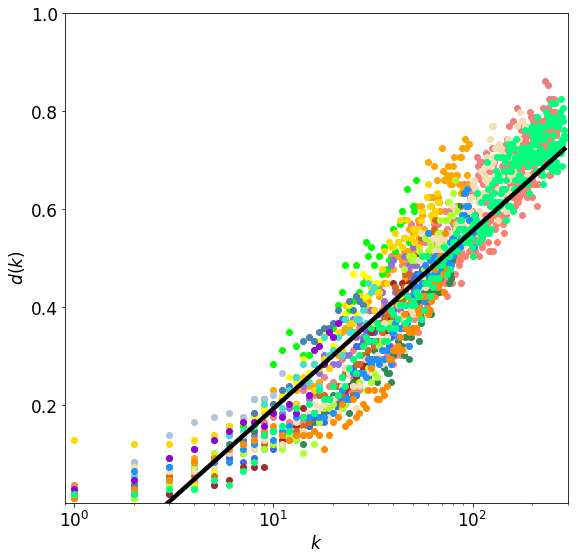
\includegraphics[scale=.45]{DR_log.png}
%		\caption{Diversidad de rango de los préstamos acumulados entre idiomas (escala logarítmica).}
%		\label{fig.DR_log} 
%	\end{minipage}
%\vspace{1pt}
%	\begin{minipage}[]{1\linewidth}
%		\centering
%		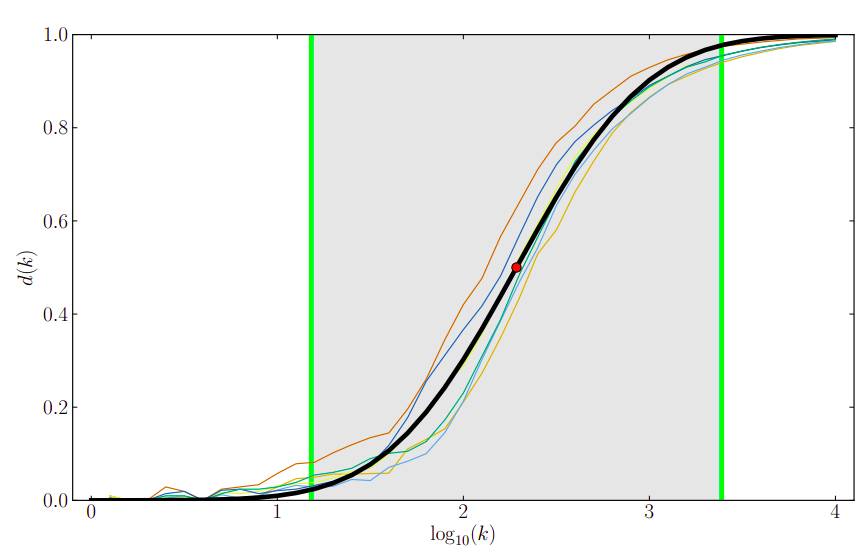
\includegraphics[width=.9\textwidth]{DR_sergio.png}
%		\caption{Diversidad de rango para distintos idiomas. }
%		\label{fig.DR_sergio}
%	\end{minipage}%
%\end{figure*}

\begin{figure}[h!]
	\centering
	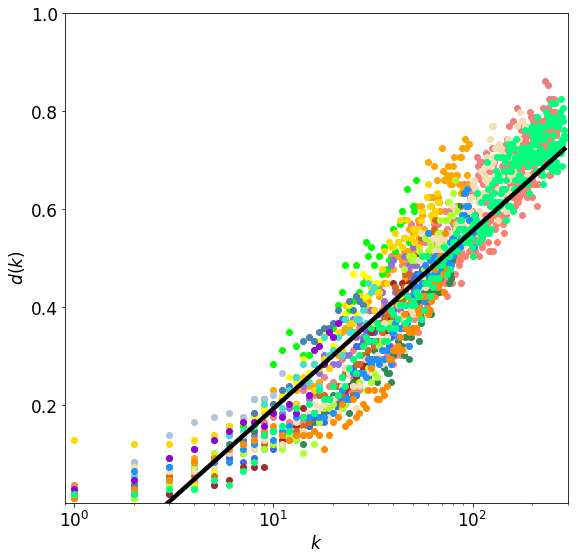
\includegraphics[scale=.38]{DR_log.png}
	\caption{Diversidad de rango de los préstamos acumulados entre idiomas (escala logarítmica).}
	\label{fig.DR_log} 
\end{figure}

\begin{figure}[h!]
	\centering
	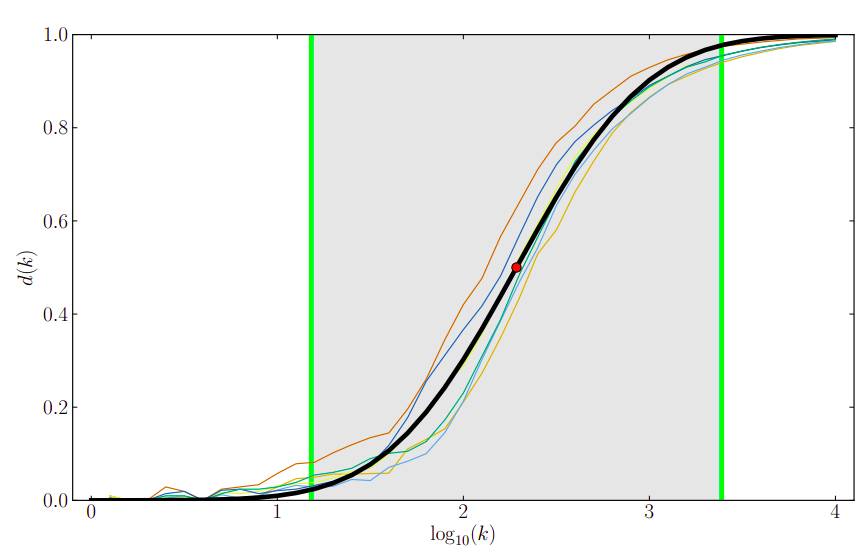
\includegraphics[width=.8\textwidth]{DR_sergio.png}
	\caption{Diversidad de rango para las palabras mas usadas de distintos idiomas. }
	\label{fig.DR_sergio} 
\end{figure}

%A pesar de que se trata de la misma conclusión de los trabajos previos, en ellos las graficas de diversidad son diferentes, obteniendo curvas de tipo sigmoide.  Una de las diferencias con los trabajos previos, 

%La principal diferencia con  los trabajos previos son los rangos donde se buscan la diversidad, estos llegan a ser del orden de $10^{4}$, mientras que en los préstamos acumulados los rangos varían entre 8 y 290. Se asocia a la escasez de rangos, el factor que en este caso determina obtener una curva logarítmica.   


\section{Resultados generales}

La diversidad de rango en los préstamos acumulados, mostró que las palabras que tienden a cambiar más su rango a lo largo del tiempo, son las que tienen rangos intermedios y bajos dentro de un ordenamiento.

También se corroboraron los resultados de diversidad previos, donde sin importar la cantidad de rangos que tenga el corpus, habrá una menor cantidad de palabras que ocupen los rangos más bajos;  y conforme aumente el rango, también lo harán las distintas palabras que lo puedan ocupar. 


 



